% small.tex
\documentclass[10pt]{beamer}
\usetheme{amcg}
\beamertemplatenavigationsymbolsempty
\renewcommand{\thefootnote}{}
\providecommand{\e}[1]{\ensuremath{\times 10^{#1}}}
\usepackage{mathptmx}
\usepackage{helvet}
\newcommand\TILDE{\char`\~}
\usepackage{listings}
\usepackage{subfigure}

% items enclosed in square brackets are optional
\title[GFD examples]{Summary of the GFD examples}
\subtitle[]{}
\institute{Department of Earth Science and Engineering, Imperial College London}
\author[Adam Candy]{\large{Adam Candy}}
\date{}

\usepackage{xstring}
\noexpandarg
\newcommand{\option}[1]{\texttt{\protect\StrSubstitute{#1}{/}{\slash}}}

\begin{document}

%--- the titlepage frame -------------------------%
\begin{frame}
  \titlepage
\end{frame}

%-- Overview slide --- %
\section*{Outline}
\begin{frame}
  \frametitle{Outline}
  \tableofcontents
\end{frame}

%-- Add sections and your outline will be created automatically --%
\subsection{The lock--exchange}

% Frame starts a new slide
\begin{frame}
    \frametitle{The lock--exchange}
\begin{itemize}
\item Fluids of different densities (temperature) separated by a barrier. As the barrier is removed, the denser fluid
  collapses under the lighter.
\item Boussinesq flow, control volume discretisation, mesh adaptivity
\item Run time: 10 min.
\end{itemize}

\begin{figure}
\centering
\includegraphics[width=0.45\textwidth]{./lock_exchange/le_basic_0_T}
\caption{Lock-exchange initial temperature (colour) distribution.}
\end{figure}

\end{frame}
%
\begin{frame}
    \frametitle{The lock--exchange}
\begin{figure}[ht]
  \centering
  % For some reason tex4ht doesn't like these images.
  \subfigure[$t = 0\,$s]{\includegraphics[width=0.45\textwidth]{./lock_exchange/le_basic_0_T}}
  \subfigure[$t = 0\,$s]{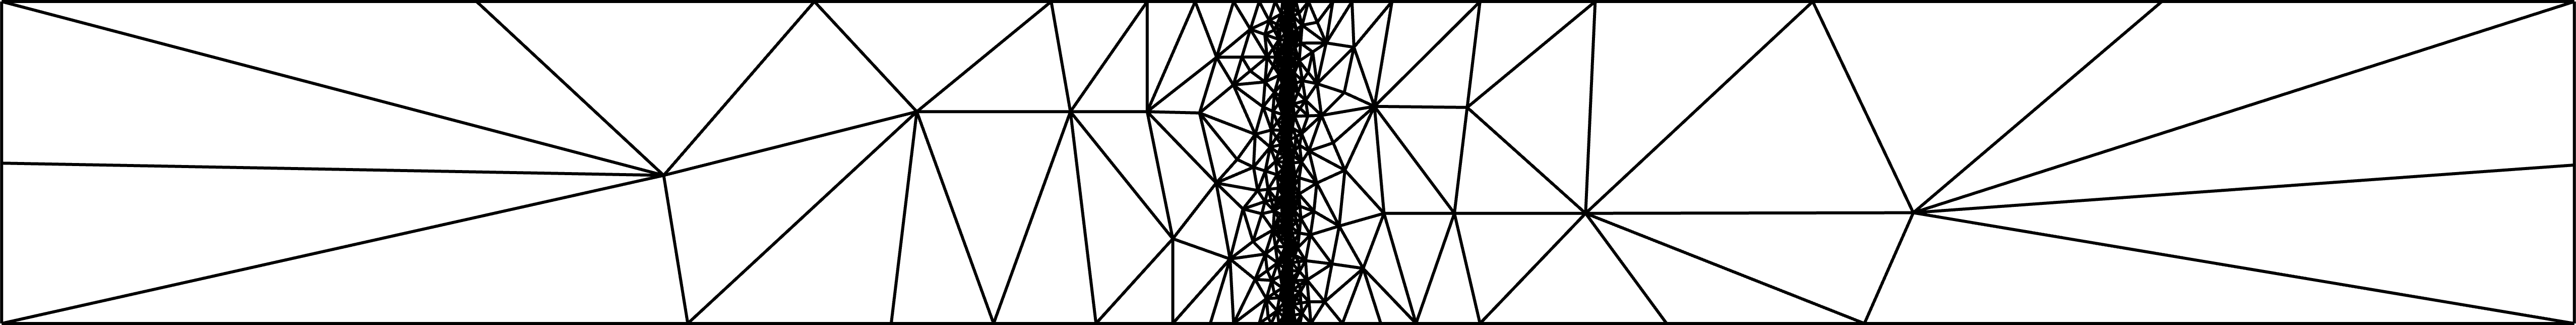
\includegraphics[width=0.45\textwidth]{./lock_exchange/le_basic_0_mesh_nice}} \\
  \subfigure[$t = 12.475\,$s]{\includegraphics[width=0.45\textwidth]{./lock_exchange/le_basic_10_T}}
  \subfigure[$t = 12.475\,$s]{\includegraphics[width=0.45\textwidth]{./lock_exchange/le_basic_10_mesh}} \\
  \subfigure[$t = 37.475\,$s]{\includegraphics[width=0.45\textwidth]{./lock_exchange/le_basic_30_T}}
  \subfigure[$t =
  37.475\,$s]{\includegraphics[width=0.45\textwidth]{./lock_exchange/le_basic_30_mesh}}
  \caption{Lock-exchange temperature distribution (colour) with meshes, over time ($t$).}
\end{figure}
\end{frame}
%
\begin{frame}
    \frametitle{The lock--exchange, diagnostics}
\begin{itemize}
\item Front speed (or Froude number)
\item Mixing given by domain fraction of fluid in specified temperature classes
\end{itemize}

\begin{figure}
\centering
\includegraphics[width=0.5\textwidth]{./lock_exchange/mixing}
\caption{Time evolution of fraction of domain that contains fluid in three temperature classes. Blue: cold, red: warm, green : mixed}
\end{figure}

\end{frame}
%
\begin{frame}
    \frametitle{The lock--exchange, exercises}
\begin{itemize}
\item Increase the simulation time from the default settings (to e.g. 30 secs) and calculate the average Froude number
\item Play with the adaptivity options.
\item Change the diffusivity and viscosity values.
\item Run with a fixed mesh (this will require making a new input mesh)
\item Try adding some detectors to visualise the particle trajectories.
\end{itemize}

\end{frame}

%-- Add sections and your outline will be created automatically --%
\section{Tsunami}

% Frame starts a new slide
\begin{frame}
    \frametitle{Hokkaido-Nansei-Oki tsunami}
\begin{minipage}[]{0.5\linewidth} 
\begin{itemize}
\item Okushiri island, Japan, 1993. 
\item Runup height of up to 30m.
\item Simulation based on a 1:400 laboratory setup.
\item Uses the free-surface and wetting and drying functionality of Fluidity.
\end{itemize}
\end{minipage}
\hspace{0.5cm}
\begin{minipage}[]{0.4\linewidth} 
\begin{figure}
\begin{center}
\includegraphics[width=\textwidth]{hokkaido-nansei-oki_tsunami/MonaiValleyDomainWithInputWave2_png.pdf}
\end{center}
\caption{The domain and the three gauge stations.}\label{fig:monai_inputwave}
\end{figure}
\end{minipage}
\end{frame}

\begin{frame}
    \frametitle{Hokkaido-Nansei-Oki tsunami}
\begin{figure}
\begin{center}
\includegraphics[width=0.7\textwidth]{hokkaido-nansei-oki_tsunami/MonaiValley_C_p1p1_nu0_01_kmkstab_drag0_002_butcircularoundisland0_2-crop-crop_final2.pdf}
\caption{The numerical and experimental results at the three gauge stations.}\label{fig:monai_results}
\end{center}
\end{figure}
% end my slide
\end{frame}


\begin{frame}
    \frametitle{Hokkaido-Nansei-Oki tsunami - Exercises}
  \begin{itemize}
    \item Add more detectors.\newline
    \item Check how increasing the wetting and drying threshold parameter affects the results.\newline
    \item Try changing the viscosity value (How does it affect the inundation of the tsunami event?).
  \end{itemize}
% end my slide
\end{frame}



%-- Add sections and your outline will be created automatically --%
\subsection{Rotating periodic channel}

% Frame starts a new slide
\begin{frame}
    \frametitle{Rotating periodic channel}
\begin{itemize}
\item Unit square domain, periodic in zonal direction and zero-slip at North and South boundaries.  Coriolis forcing.
\item The flow is driven by a velocity source term:
\begin{equation*}
  \vec{F}=
  \begin{bmatrix}
    y^3 \\
    0
  \end{bmatrix}
\end{equation*}
\item Provides a convergence test for the $P_{1DG}P_2$ element pair.
\item A good example of using python state for online diagnostics and analysis, and also using python for setting initial conditions.
\item Run time: 10 min. 
\end{itemize}
\end{frame}
%
\begin{frame}
    \frametitle{Rotating periodic channel}
\begin{figure}
\includegraphics[width=0.6\textwidth]{./rotating_channel/analytic_solution}
\caption{Velocity forcing term and analytic solutions for velocity and pressure for the rotating periodic channel test case. Note that each of these quantities is constant in the x direction.}
\end{figure}
\end{frame}
%
\begin{frame}
    \frametitle{Rotating periodic channel}
\begin{figure}
\includegraphics[width=0.6\textwidth]{./rotating_channel/convergence}
\caption{Error in the pressure and velocity solutions for the rotating channel as a function of resolution.}
\end{figure}
\end{frame}
%
\begin{frame}
    \frametitle{Rotating periodic channel, exercises}
\begin{itemize}
\item Understand the use of analytic forcing functions in Fluidity using Python.
\item For the Continuous Galerkin example, see what the effect is of removing the SUPG stabilisation
\item Change the resolution of the adapted meshes
\item Change the spatial and temporal discretisations to get a less diffusive advection scheme
\end{itemize}
\end{frame}


%-- Add sections and your outline will be created automatically --%
\section{Restratification after open-ocean deep convection}

\begin{frame}
    \frametitle{Restratification - Setup}
\begin{itemize}
    \item This example is an idealised model of the restratification phase of open-ocean deep convection (OODC).
    \item The setup is taken from Rousset et al. [2009].
    \item Cylinder, radius 250km, height 1km.
\end{itemize}
\begin{figure}
\centering
\includegraphics[width=0.4\textwidth]{./restratification_after_oodc/rousset-init.png}
\caption{Cross section of initial temperature distribution.}
\end{figure}
\end{frame}

\begin{frame}
    \frametitle{Restratification - Output}
\begin{figure}
\begin{center}
\subfigure [10 days]{\includegraphics[width=0.2\textwidth]{./restratification_after_oodc/rousset-res5000-depth-40m0003.png}}
\hspace{1cm}
\subfigure [20 days]{\includegraphics[width=0.2\textwidth]{./restratification_after_oodc/rousset-res5000-depth-40m0005.png}}

\subfigure [30 days]{\includegraphics[width=0.2\textwidth]{./restratification_after_oodc/rousset-res5000-depth-40m0007.png}}
\hspace{1cm}
\subfigure [40 days]{\includegraphics[width=0.2\textwidth]{./restratification_after_oodc/rousset-res5000-depth-40m0009.png}}
\caption{The temperature cross-section at a depth of 40m.}
\label{fig:rousset-40m}
\end{center}
\end{figure}\end{frame}

\begin{frame}
  \frametitle{Restratification - Exercises}
\begin{itemize}
\item How does mesh adaptivity influence the solution?
\item Fixed mesh resolution size - what happens as you increase/decrease the resolution?
\item Discretisation of temperature - what changes between DG, CG and CV?
\item Scaling - how far can you push the parallisation of this run, with and without adaptivity?
\end{itemize}
\end{frame}







%-- Add sections and your outline will be created automatically --%
\section{Tides in the Mediterranean Sea}

% Frame starts a new slide
\begin{frame}
    \frametitle{Tides in the Mediterranean Sea}
\begin{itemize}
\item Tidal modelling is a widely used method for validating free surface implementations.
\item Tides introduced by an astronomical body forcing, and a
\item Co--oscillating boundary tide forcing.
\item This example considers the four main tidal constituents: \mbox{$M_2, \, S_2, \, K_1 \,\, {\rm and} \,\, O_1$}.
\end{itemize}
\end{frame}
%
\begin{frame}
    \frametitle{Tides in the Mediterranean Sea}
\begin{figure}
\centering
\includegraphics[width=0.9\textwidth, clip = True, trim = 5mm 180mm 0mm 0mm]{./tides_in_the_Mediterranean_Sea/amp.png}
\caption{The $M_2$ tidal harmonic amplitude from (left) Fluidity--ICOM and (right) a high resolution tidal model${}^\dagger$.}
\end{figure}
\footnote{${}^\dagger$ M.~N.~Tsimplis {\it et al.} (1995), J. Geophys. Res. 100 (C8).}
\end{frame}
%

\begin{frame}
    \frametitle{Tides in the Mediterranean Sea}
The amplitude of each of the todal components is considered, and a RMS error of the difference of these to observed tide guage data is calculated.  The locations of these tide guages is shown below.
\begin{figure}
\centering
\includegraphics[width=0.6\textwidth]{./tides_in_the_Mediterranean_Sea/gauges.png}
\caption{Locations of 62 tide gauges in the Mediterranean Sea used to calculate the root mean square error.}
\end{figure}
\end{frame}


\begin{frame}
    \frametitle{Tides in the Mediterranean Sea - exercises}
\centering
\begin{itemize}
\item Consider the forcing tidal components contained in the netCDF file 'med.nc' (e.g. using ncview).
\item Examine the mesh features (e.g. open the '.msh' file in Gmsh).
\item Look at how to apply the forcing of different tidal components in the simulation.
\item Limit the error calculation by region, are the errors greater in some parts of the Mediterranean?
\end{itemize}
\end{frame}

\section{Setting up simulations of geophysical processes}

\begin{frame}{Setting up simulations of geophysical processes, an overview}
\begin{columns}[l]

\column{3.5in}
The following aspects will be outlined:
  \begin{itemize}
     \item Meshing 
        \begin{itemize}
        \item[$\circ$] Gmsh is used to produce a mesh on a spherical manifold,
        \item[$\circ$] An extrusion, creating a 3D mesh is carried out within fluidity,
              controlled by options in Diamond.
     \end{itemize}
     \item Additional options in Diamond for:
     \begin{itemize}
        \item[$\circ$] Gravity force,
        \item[$\circ$] Coriolis pseudo-force,
        \item[$\circ$] Bottom drag,
        \item[$\circ$] Free surface,
        \item[$\circ$] Tidal forcing.
     \end{itemize}

  \end{itemize}

%Example available in directory:\\
%{\it trunk/examples/tides\_in\_the\_Mediterranean\_Sea}

\column{1.5in}
\vspace{-0.4in}
\begin{figure}[htbp!]
 \centering
  \includegraphics[width=0.9\textwidth]{./tides_in_the_Mediterranean_Sea/figures/globe_mesh}
\end{figure}

\end{columns}

\end{frame}

\begin{frame}{2D horizontal mesh}

\begin{figure}[htbp!]
 \centering
  \includegraphics[width=0.6\textwidth]{./tides_in_the_Mediterranean_Sea/figures/med_mesh2}
\end{figure}
\begin{itemize}
\item Mesh is generated on a spherical shell using Gmsh.
\\ Tutorial {\footnotesize \url{http://amcg.ese.ic.ac.uk/files/gmsh\_tutorial.pdf}} or \\ {\footnotesize \url{http://perso.uclouvain.be/jonathan.lambrechts/gmsh_ocean/}}
\item Coastlines extracted from the GSHHS dataset.
\item Mesh available in {\it trunk/examples/tides\_in\_the\_Mediterranean\_Sea/med.msh}
\end{itemize}

\end{frame}

\begin{frame}{Extruding in Fluidity}
\begin{itemize}
\item 2D horizontal mesh is extruded vertically within Fluidity at runtime.
\end{itemize}
\begin{figure}[htbp!]
 \centering
  \includegraphics[width=1.0\textwidth]{./tides_in_the_Mediterranean_Sea/figures/mesh_extrusion.png}
\end{figure}
\begin{itemize}
\item Flexibility to choose layered $\sigma$ or $z$--coordinates.
\item Bathymetry extracted from a NetCDF file ({\it e.g.} $GEBCO$ dataset).
\end{itemize}

\begin{figure}[htbp!]
 \centering
  \includegraphics[width=0.3\textwidth]{./tides_in_the_Mediterranean_Sea/figures/extrude}
\end{figure}

\end{frame}

\begin{frame}{Extrusion: Representation of the surface of the spherical Earth}
\begin{itemize}
  \item Linear mapping
  \begin{itemize}
    \item[$\circ$] Element faces on sea surface are flat,
    \item[$\circ$] Appropriate choice for P1 grids,
    \item[$\circ$] Suitable for barotropic simulations.
  \end{itemize}
  \item Super--parametric mapping
  \begin{itemize}
    \item[$\circ$] Element faces on sea surface are described by $n^{th}$ order polynomials,
    \item[$\circ$] Order of polynomial equal to the degree of the mesh,
    \item[$\circ$] Suitable for baroclinic simulations (currently up to 2nd order in parallel).
  \end{itemize}
\end{itemize}

\end{frame}

\begin{frame}{Gravity, Coriolis and bottom drag}
\begin{itemize}
  \item Gravity force and Coriolis pseudo-force are set under physical parameters
  \begin{itemize}
    \item[$\circ$] Gravity magnitude and direction,
    \item[$\circ$] Coriolis ($f$--, $\beta$--plane, on-sphere).
  \end{itemize}
  \item Ocean floor: no-normal-flow \& drag wall-law
  \begin{align*}
  \frac{\partial u}{\partial z} \propto D_{bottom} = \frac{1}{2} C_D \rho u^{2},
  \end{align*}
  set as boundary condition on velocity:
\end{itemize}
\begin{figure}[htbp!]
 \centering
  \includegraphics[width=0.6\textwidth]{./tides_in_the_Mediterranean_Sea/figures/bottom_drag}
\end{figure}
\end{frame}

\begin{frame}{Setting the free surface}
\begin{itemize}
  \item Free surface - kinematic boundary condition on velocity.
  \begin{itemize}
    \item[$\circ$] The velocity of a particle at the surface is tangential to the surface.
  \end{itemize}
\end{itemize}

\begin{columns}[l]
\column{2.5in}
  \begin{align*}
    -\overrightarrow{n}_s \cdot \overrightarrow{n}_g\frac{\partial h}{\partial t} = \overrightarrow{n}_s \cdot \overrightarrow{u}
  \end{align*}

\column{2.5in}
  \begin{figure}[htbp!]
   \centering
    \includegraphics[width=0.8\textwidth]{./tides_in_the_Mediterranean_Sea/figures/free_surface}
  \end{figure}
\end{columns}

\begin{figure}[htbp!]
 \centering
  \includegraphics[width=0.6\textwidth]{./tides_in_the_Mediterranean_Sea/figures/freesurface}
\end{figure}

\end{frame}

\begin{frame}{Setting the tidal forcing-body forcing}
  \begin{itemize}
  \item Astronomical body forcing.
    \begin{itemize}
       \item[$\circ$] Specify the tidal components.
    \end{itemize}
  \end{itemize}
  \begin{figure}[htbp!]
    \centering
    \includegraphics[width=0.7\textwidth]{./tides_in_the_Mediterranean_Sea/figures/body_forcing}
  \end{figure}
\end{frame}

\begin{frame}{Setting the tidal forcing-free surface elevation at boundary}
  \begin{itemize}
  \item Dirichlet boundary condition on pressure at open boundaries.
    \begin{itemize}
       \item[$\circ$] Pressure set for free-surface elevation to match observational data.
    \end{itemize}
  \item User has to specify:
    \begin{itemize}
       \item[$\circ$] Which tidal components,
       \item[$\circ$] NetCDF file to read free-surface elevation from,
       \item[$\circ$] Name of phase and magnitude variables in file.
    \end{itemize}
  \end{itemize}
  \begin{figure}[htbp!]
    \centering
    \includegraphics[width=0.6\textwidth]{./tides_in_the_Mediterranean_Sea/figures/diamond_freeSurf_pre_Bc.png}
  \end{figure}
\end{frame}



%-- Data directory slide --- %
\section*{Data}
\begin{frame}
  \frametitle{Data}
  \begin{center}
  The examples have been run in advance \\ and the output can be found in \\
  \vspace{1cm}
  /scratch/Training2012/
  \end{center}
\end{frame}

\end{document}




